\begin{block}{Approach}
\centering

%\begin{block}{Quantity of Interest Map}
\centering
\vspace{1cm}
\heading{Quantity of Interest Map}
    \emph{\large A Functional Relating \textbf{Predictions} and \textbf{Data}}
    \large
    \begin{itemize}
       \itembox{Ideal} $Q \left (\param, \noise \right ) = F \left ( \obs(\param), \data(\noise) \right )$
       \itembox{Theoretical} $Q \left ( \pspace, \nspace \right ) =: \dspace_\mathcal{T} \subset \RR$
       \itembox{Practical} $\widehat{Q} \left (\param \right ) = F \left ( \obs(\param), \data^\dagger \right )$
       \itembox{Computable} $\widehat{Q} \left ( \pspace \right ) =: \dspace_\mathcal{C} \subset \dspace_\mathcal{T}$
    \end{itemize}
    \begin{figure}
        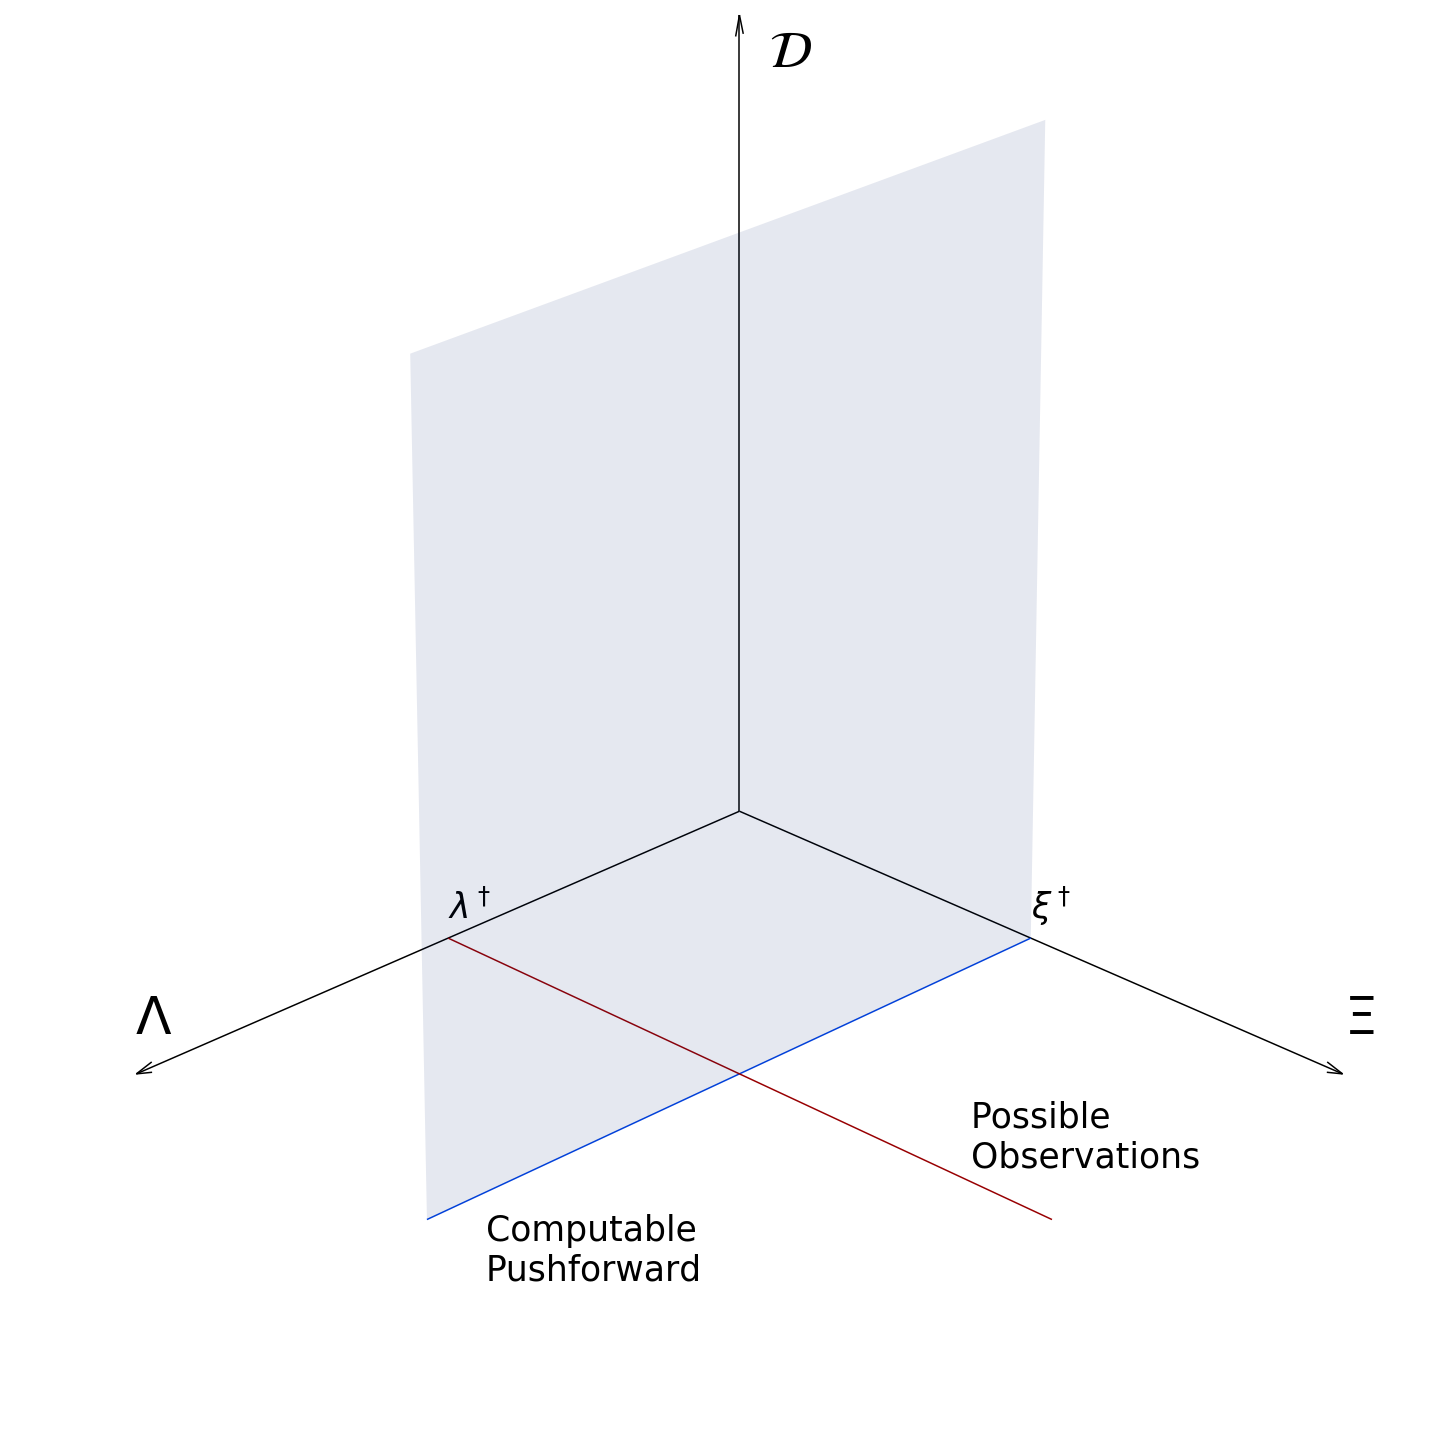
\includegraphics[height=23cm]{diagram}
    \caption*{\large \emph How do conditionals of $\nspace$ compare to the joint density?}
    \end{figure}


\heading{Observed Distribution}
{\large \emph Given a functional, what measure do we invert?}

\Large
    $Q(\param^\dagger, \noise) \sim \observed$ when we allow $\noise$ to vary over $\nspace$
%\vspace{1cm}
    \begin{table}
      \centering
      %{\setlength{\extrarowheight}{15pt}i
      {\setlength{\tabcolsep}{0.25em}
      \begin{tabular}{c <{\hspace{1pc}} c >{\hspace{1pc}} c}
        %\toprule
        %\large
        \textbf{$F(\obs, \data^\dagger)$} & \textbf{$\noise$} & {$\observed$} \\
        \midrule
        $\frac{1}{\sigma\sqrt{D}} \large\sum \left( \obs_i\lam - \data_i^\dagger \right)$ & $ \noise \sim L^2$ & $N(0,1) $ \\[1.5ex]
        $\frac{1}{\sigma^2} \large\sum \left ( \obs_i\lam - \data_i^\dagger \right)^2$ & $ \noise \sim N(0,\sigma^2) $ & $\chi^2 (D)$ \\[1.5ex]
        $\frac{1}{\sigma^2 D} \large\sum \left ( \obs_i\lam - \data_i^\dagger \right)^2$ & $ \noise \sim N(0,\sigma^2) $ & $ \Gamma \left ( D/2, D/2) \right ) $ \\
        \normalsize\vdots & \normalsize\vdots & \normalsize\vdots \\
        %\bottomrule
      \end{tabular}
      }
      \caption*{Choices of $F$ and associated $\observed$ for stochastic inverse problem}
    \end{table}

%    \begin{figure}
%        \includegraphics[width=15cm]{converge}
%        \caption{$\observed$ compared to $Q(\param^\dagger,\noise)$ for $D=1$.}
%    \end{figure}
%
\end{block}
